% #region PREAMBEL OG PAKKER
\documentclass[a4paper, 12pt]{article}  % DOKUMENTKLASSE
\title{Eksamen ØKO1001\\Del 1: Ledelse} % TITTEL
\author{Kandidatnr. 10026}              % FORFATTER
\date{\today}                           % DATO & FAG

\usepackage[english, norsk]{babel}      % NORSK SPRÅK
\usepackage[                            % BIBLIOGRAFI
    backend=biber,
    style=apa,
    ]{biblatex}
\usepackage{csquotes}                   % PAKKE TIL BABEL
\addbibresource{ref.bib}                % PATH TIL BIBLIOGRAFI
\usepackage[hidelinks]{hyperref}        % LENKER I TOC OG GENERELT
\usepackage[margin=1in]{geometry}       % VANLIG STØRRELSE MARGIN
\setlength{\parindent}{0em}             % SKILLER AVSNITT
\setlength{\parskip}{1em}               % SKILLER AVSNITT
\usepackage{setspace}
\setstretch{1.4}                        % 1.5 LINJEAVSTAND
\usepackage{graphicx}                   % BILDER \includegraphics[OPTIONS]{PATH}
\usepackage{kantlipsum}                 % FYLLTEKST I KANT-STIL (kant[n-m])
\usepackage{amsfonts}                   % BLACKBOARD BOLD FONT (\mathbb{N})
\usepackage{import}                     % IMPORTER FILER (\import{PATH}{FILE})
\usepackage{caption}                    % PAKKE FOR BEDRE CAPTIONS I FIGURER
\usepackage{float}                      % FLYTT FIGURER 
\usepackage{booktabs, multirow} % for borders and merged ranges
\usepackage{soul}% for underlines
\usepackage[table]{xcolor} % for cell colors
\usepackage{changepage,threeparttable} % for wide tables
% #endregion
\begin{document}
% #region INNHOLDSFORTEGNELSE
\maketitle
\vfill
\begin{center}
  ØKO1001 - Ledelse
\end{center}
\thispagestyle{empty}
\addtocounter{page}{-1}
\newpage
\tableofcontents % INNHOLDSFORTEGNELSE
\thispagestyle{empty}
\addtocounter{page}{-1}
% #endregion
\newpage
\section{Quiet quitting og ledelse?}

\subsection{Hva er ``Quiet quitting''?}

Quiet quitting er en trend fra USA som har spredt seg som ild i tørt gress i sosiale medier, og særlig på plattformen TikTok. 
Ifølge Bergens Tidene har emneknaggen \texttt{\#quietquitting} over 274 millioner treff på TikTok \parencite{bt22}, og fenomenet har også tatt veien til Norge. 
Quiet quitting går kort fortalt ut på at man som arbeidstaker ønsker å ha et klart og tydelig skille mellom arbeid og fritid, 
``\emph{Gjør jobben din, å dra hjem}'' omtaler Sigrid Sollund det som i Dagsnytt 18 \parencite{dax18}.

Fenomenet er populær bland generasjon Z, unge arbeidstakere født fra slutten av 90-tallet til rundt 2010, 
og det er kanskje også derfor den florer på sosiale medier i de plattformene de unge brukes mest.
Det er derimot ikke bare de unge som følger trenden, i følge amerikansk gallup er halvparten av de ansatte i USA såkalte ``quiet quitters'' \parencite{dax18}.

Det ironiske med quiet quitting er nettopp det at det har sitt utspring fra USA; landet der man skal kunne få til alt man vil. 
Den amerikanske drømmen går ut på at hvem som helst kan få til hva som helst, så lenge man jobber hardt nok. 
Amerikaneren Frank Sinatra sier det best selv ``\emph{If I can make it there, I'll make it anywhere}''. 
Tar man quiet quitting på kornet kan det heller minne om Aksel Sandemoses Jantelov, ``\emph{Du skal ikke tro at du \emph{er} noe}'', og kanskje er det derfor det også har slått ann i Norge.

\subsection{Er Quiet quitting et problem for ledere?}

1000kr spørsmålet er da om dette er et problem for lederne? 
Trenger de i det hele tatt å bry seg om at alle ikke vil legge inn det lille ekstra, og gi litt mer innsats enn de trenger? 
Vel, det kan avhenge veldig ut i fra hva slags leder man er. 
Hvis vi tar utgangspunkt i Blake og Moutons \emph{ledergitter} (Figur \ref{fig:ledergitter}) ser vi rammeverket for fem forskjellige ledere.

Alle disse fem ledertypene vil ha et anderledes forhold til en quiet quitter. 
La oss starte med å ta utgangspunkt i ledertypen nederst til venstre i gitteret, ``La-det-skure''-lederen.

\begin{figure}[H]
  \centering
  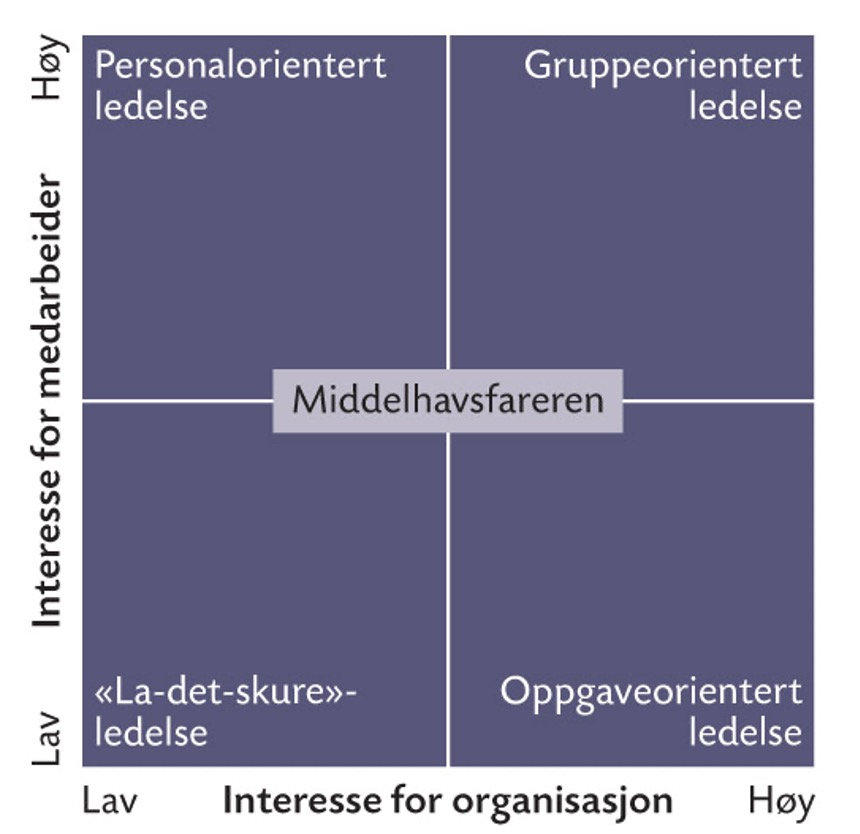
\includegraphics[width=8cm]{img/ledergitteret.jpg}
  \caption{Ledergitteret \parencite[63]{ledelse}}
  \label{fig:ledergitter}
\end{figure}

En leder som følger \emph{``La-det-skure''-ledelse} vil neppe føle noen store problemer eller utfordringer med en quiet quitter. 
Lederen bryr seg nemlig i praksis lite om medarbeiderne og like lite om bedriftens resultater \parencite{ledelse}. 
At en medarbeider bare gjør akkurat det de blir bedt om og ikke noe mer er jo midt i blinken! 
``Hva skal jeg si, du gjør jo akkurat det du får beskjed om, hva annet kan jeg forvente!'' kan man tenke seg lederen vil si under en medarbeidersamtale.

Den rake motsetningen finner vi ikke overraskende i motsatt felt i gitteret, den \emph{gruppeorienterte} lederen; 
en leder som er veldig motivert til å oppnå gode resultater, og motivere sine medarbeidere. 
Her kan det oppstå store gnister under en medarbeidersamtale med en quiet quitter. 
Lederen kan oppfatte medarbeideren som lat og uinteressert, og medarbeideren kan oppfatte lederen som påtrengende og slitsom.

I samme båt, men på hver sin ende, finner vi den \emph{personalorienterte} og den \emph{oppgaveorienterte} lederen. 
Disse lederne vil oppleve liknende utfordringer som den gruppeorienterte lederen, men må håndtere de ulikt. 
Den personalorienterte lederen vil kunne oppleve medarbeideren uinteressert i unødvendig samarbeid, mens den oppgaveorienterte lederen kan oppfatte medarbeideren som litt umotivert, og tilbakeholden. 

Til sist, men ikke minst, har vi \emph{middelhavsfareren}; ledernes Medel-Svensson, Ola Nordmann og John Doe i en og samme person. 
Som navnet, og plasseringen i gitteret, tilsier, ligger denne lederen å farer midt i mellom alle de andre ledertypene. 
Han padler rundt i ``de konfliktskyes sjø'', og prøver å få alle samlet på ``kompromissens øy''. 
Middelhavsfareren kan nok til tider også oppleve en quiet quitter som litt utfordrende, men prøver nok rast og ikke gjøre det for vanskelig for seg selv og lar de holde på som de vil.

\subsection{Hvordan skal en leder møte en Quiet quitting?}

Ledergitteret i Figur \ref{fig:ledergitter} er ikke en oppskrift på perfekt ledelse. 
For som Hersey og Blanchard hevder er det ikke én lederstil som er perfekt, og kan brukes i alle typer situasjoner \parencite{ledelse}. 
Dette gjelder også vår quiet quitter. 
En effektiv og god leder er en som kan tilpasse seg situasjonen en er i, og de menneskene man jobber med. 

\begin{figure}[H]
  \centering
  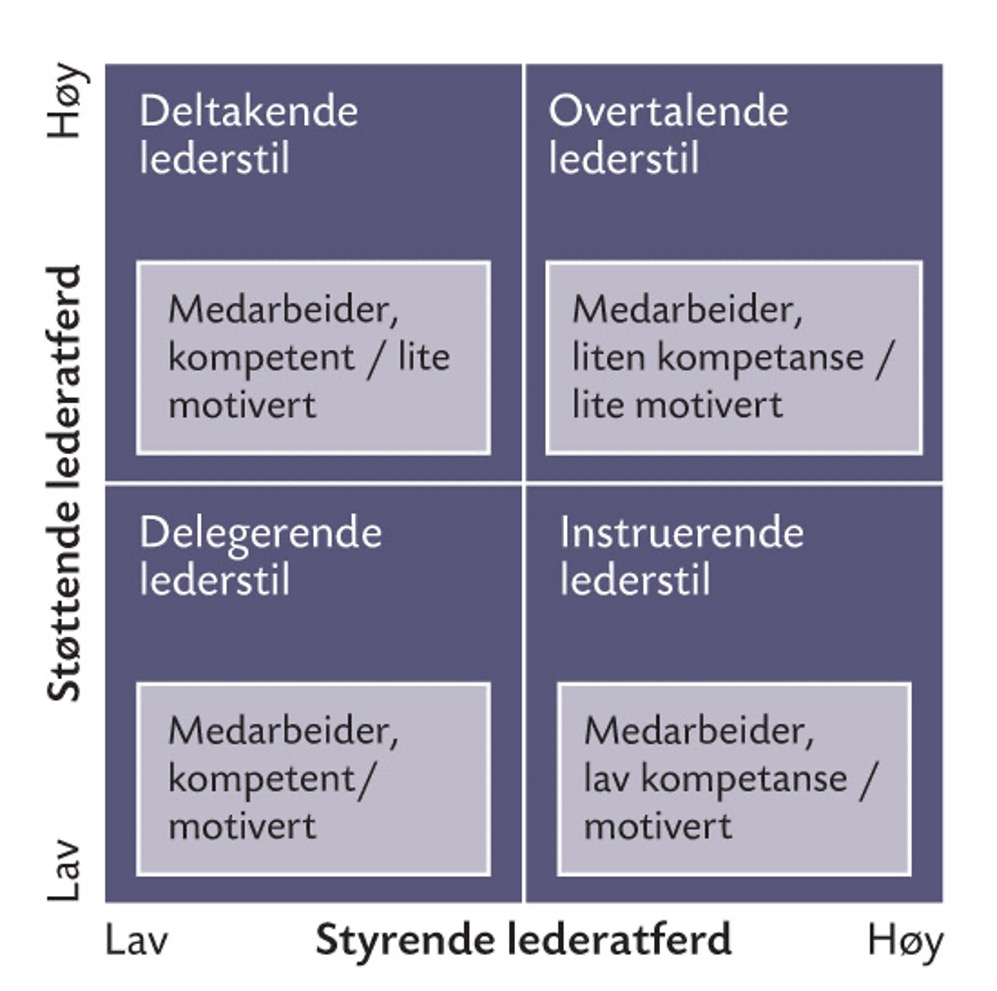
\includegraphics[width=8cm]{img/situasjonsbestemt.jpg}
  \caption{Situasjonsbestemt ledelse \parencite{ledelse}}
  \label{fig:situasjon}
\end{figure}

\emph{Situasjonsbestemt ledelse} går ut på å nettopp dette å tilpasse seg til situasjonen man er i. 
I Figur \ref{fig:situasjon} ser vi i hvilke situasjoner de ulike stilene faller til. 
Det første steget for en leder i møte med en quiet quitter er da å identifisere hvor i rubrikken medarbeideren faller, og tilpasse sin stil etter det. 

Felles for de fleste som driver med quiet quitting er motivasjonen. 
Det blir kanskje ikke nødvendig vis helt riktig å si at alle er lite motivert for arbeidet, men det vi med sikkerhet kan si er at de er svært lite motivert til å jobbe utover det de mener de er pliktig.
Med tanke på Figur \ref{fig:situasjon} blir det da riktig å si at de faller innenfor øvre del av tabellen.
Den andre aksen er ikke like lett å generalisere blant quiet quitters; holdningen deres reflekterer ikke nødvendig vis noe om hvilken kompetanse de har i feltet sitt. 
Noen kan være godt kompetente men ha et ønske om å ikke ta med seg arbeidet til middagsbordet, mens andre bare vil prøve å være anonyme og skjule at de har manglende kompetanse.
Da ser vi at lederen må være tilpasningsdyktig og enten deltakende og motiverende, eller overtalende og bestemt. 
Her er det også viktig å merke seg at med overtalende menes ikke autoritær og streng; det vil trolig bare forverre situasjonen.
En overtalende leder må klare å oppmuntre medarbeideren og være støttende arbeidet så de føler jeg kompetente og verdsatt.
Det handler i stor grad om å kunne ha en god kommunikasjon og snakke \emph{med}, ikke \emph{til} kollegaen.


\subsection{Hvordan leder man en Quiet quitter?}

Til nå har vi funnet ut hvordan ulike ledertyper kan oppleve en quiet quitter, og hvordan man skal håndtere å møte en. 
Men hva slags leder vil man, eller bør man være, hvis man vil være en god leder for en quiet quitter? 
Hvilken lederstil skal man sikte seg inn på?

For å finne ut hva man skal velge er det enkleste å først legge på bordet hva som trolig ikke vil fungere. 
Å være autoritær har allerede blitt nevnt, og det er nesten innlysende. 
En som ikke brenner for jobben og helst bare vil se på den som en nødvendighet for å få hjulene til å gå rundt, vil bare bli enda mindre motivert og inspirert hvis lederen krass, streng og urettferdig.
Denne må man klart styre unna.

Hva nå med ``La-det-skure''-lederen? 
Vi har allerede sett at denne lederen ikke var så engstelig for å jobbe med en quiet quitter, så kanskje det ligger en likesinnet kjærlighet mellom de? 
Trolig vil ikke noen av partene ha det vanskelig med hverandre, og kanskje til og med trives ganske godt i lag. 
For bedriftens del går det nok ikke derimot ikke like plettfritt.
En dårlig egnet leder, og ansatte som holder unna å gi det lille ekstra, klarer kanskje å holde en etablert bedrift flytende i gode tider, men det er nok kanskje også det beste de greier.

Den siste lederstilen jeg vil dra fram som kan være utfordrende i denne situasjonen er verdibasert ledelse; en stil som i de fleste andre tilfeller virkelig kan motivere ansatte. 
Problemet her er nok at ved å være en quiet quitter har man allerede innstilt seg på at jobben bare er en dyd av nødvendighet.
Å spille på bedriftens verdier og samfunnsoppdrag hjelper da ikke særlig mye, siden den ansatte har utstrålt at sine verdier handler mer om at de kan være fri, enn at bedriftens får til det den trenger.
Denne er ikke et like dårlig valg som de to første, og kan i enkelte tilfeller, der alt den ansatte trenger bare er litt ekstra motivasjon, fungere, men den er nok ikke alltid en fulltreffer.

Men hva er det nå da som kan fungere? 
En ting man kan prøve er å akseptere ``byttehandelen'' medarbeideren inviterer til definere og bli enige om veldig klare og presise arbeidsoppgaver.
På denne måten kan du som leder skape et sterkt tillitsbånd til medarbeideren som, så lenge det går begge veier, kan få medarbeideren til å føle mer frihet i arbeidet da de det akkurat hva de skal gjøre og hva som forventes av dem. 
Dette blir en form for \emph{tillitsbasert ledelse} der du som leder viser at du har tillit til at medarbeideren skal og har riktig kompetanse til å gjøre det de skal. 
Medarbeideren blir mye mer selvstendig og får tillit til å lede seg selv, såkalt \emph{selvledelse}.
I beste fall kan man få ut av denne ``handelen'' at medarbeideren får mye mer engasjement i arbeidet, og viser interesse til å yte det lille ekstra. Denne byttehandelen eller ``transaksjonen'' kan vi kalle for \emph{transaksjonsledelse}.

Hvis man vil holde seg til litt mer tradisjonelle lederstiler, eller ikke har tilliten til at en radikal endring i ledelsen er riktig valg, kan \emph{transformasjonsledelse} være løsningen. 
Transformasjonsledelse bygger litt på det vi har vært innom tidligere og tar inn elementer fra både transaksjonsledelse og verdibasert ledelse, og kombinerer de på den slik måte at medarbeideren både får litt av friheten og byttehandelen fra transaksjonsledelsen samtidig som lederen prøver transformere eller omdanne medarbeideren motivasjon gjennom virksomhetens visjoner og verdier. 
Dette kan være nøkkelen til å motivere og engasjere medarbeideren til å av og til gi det lille ekstra og yte litt mer, så lenge de ser at de får noe tilbake for all innsatsen. 
Men om det endrer innstillingen og drømmen til den ansatte om å gi slipp på arbeidets plikter, er bare opp til den ansatte.

Og kanskje var det nettopp det å gi slipp på arbeidets plikter som var Sinatras amerikanske drøm, ``\emph{Start spreading the news, I'm leaving today}''. Alt han ville var å være fri å gjøre det han ville uten å engste seg over alle andre bekymringer, ``\emph{I want to be a part of it: New York, New York}''.

\newpage
\section{Truer Quiet quitting organisasjonskulturen?}

\subsection{Hva differensierer en Quiet quitter fra andre ansatte?}

\subsection{Skal man velge yrke etter lønn eller interesse?}

\newpage
\printbibliography[heading=bibintoc] % LAGER BIBLIOGRAFI

\end{document}
